% Introduction to what a Packet storage is. Discuss its strcuture.
% Where is it used, and how is it useful.
% How many controllers it has (and why)
% What is in the report (section-wise)

The project described in this report discusses the design and verification of a small packet storage system. The packet storage system is inspired by the distributed controller of an operational product manufactured by Vanderlande, a Dutch company. 
The aim of this project is to understand and formulate the requirements of such a system, design the system and in the end verify that the system would meet the proposed requirements when in operation under different circumstance.

The packet storage system consists of two conveyor belts, one for receiving a packet into the system and the other for delivering the packet out of the system. The system consists of several racks where packets can be stored. The packets are stored by means of two elevator platforms (situated serially, one above the other). Moreover, there are five controllers in the system which run in parallel. Figure \ref{fig:packet_storage} shows the diagram of such a system. The controller C1 controls the input conveyor belt, controller C2 controls the output conveyor belt, conveyor C3 and C4 operate its respective elevators and controller C5 keeps track of all the information about racks, packet storage and its dispatch.

\begin{figure}[h]
\center
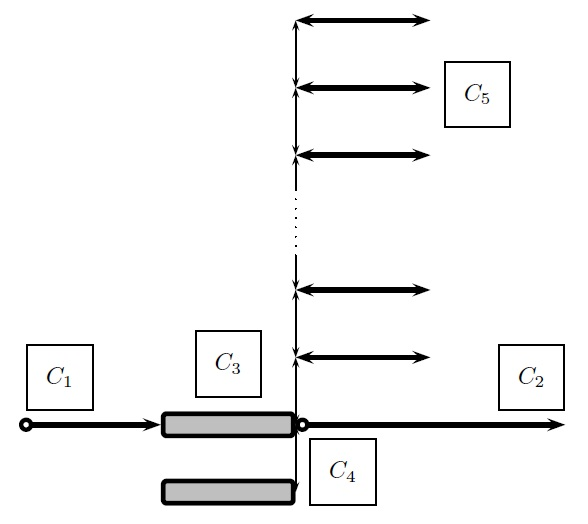
\includegraphics[width=0.6\textwidth]{packet_storage_diag}
\caption{Packet storage system, courtesy \cite{problem_statement}}
\label{fig:packet_storage}
\end{figure}

There are however, certain constraints to be understood for the given system. For example, the number of packets on the conveyor belt, rack slots and elevator platform can store at most one packet at a time, etc. Further constraints are discussed in the next section under global requirements.

The sections described in the report are the global requirements, external interactions in the system, translated requirements, the architecture of the system transpired, discussion on controllers with its labelled transition diagram(LTS) and finally discuss the verification of its global requirements.
The system is to be modelled to be intelligent to fulfil the basic requirements desired from such a system.